% Latex template: mahmoud.s.fahmy@students.kasralainy.edu.eg
% For more details: https://www.sharelatex.com/learn/Beamer

\documentclass[aspectratio=1610]{beamer}					% Document class

\setbeamertemplate{footline}[text line]{%
  \parbox{\linewidth}{\vspace*{-8pt}Dynamics on gene networks \hfill\insertshortauthor\hfill\insertpagenumber}}
\setbeamertemplate{navigation symbols}{}

\usepackage[english]{babel}				% Set language
\usepackage[utf8x]{inputenc}			% Set encoding

\mode<presentation>						% Set options
{
  \usetheme{default}					% Set theme
  \usecolortheme{default} 				% Set colors
  \usefonttheme{default}  				% Set font theme
  \setbeamertemplate{caption}[numbered]	% Set caption to be numbered
}

% Uncomment this to have the outline at the beginning of each section highlighted.
%\AtBeginSection[]
%{
%  \begin{frame}{Outline}
%    \tableofcontents[currentsection]
%  \end{frame}
%}

\usepackage{graphicx}					% For including figures
\usepackage{booktabs}					% For table rules
\usepackage{hyperref}	
\usepackage{tikz-network}				% For cross-referencing
\usepackage[absolute,overlay]{textpos}
\usepackage{bm}
\usepackage[font=small,labelfont=bf]{caption}

\title{Isolating the perturbation response of gene regulatory networks in the presence of biological variability and technical noise}	% Presentation title
\author{Clayton W. Seitz}								% Presentation author
\date{\today}									% Today's date	

\begin{document}

% Title page
% This page includes the informations defined earlier including title, author/s, affiliation/s and the date
\begin{frame}
  \titlepage
\end{frame}

\begin{frame}{Outline}
  \tableofcontents
\end{frame}


% The following is the most frequently used slide types in beamer
% The slide structure is as follows:
%
%\begin{frame}{<slide-title>}
%	<content>
%\end{frame}

\begin{frame}{Gene expression can be non-constitutive}


\begin{textblock*}{7cm}(0.5cm,1.5cm)
\begin{figure}
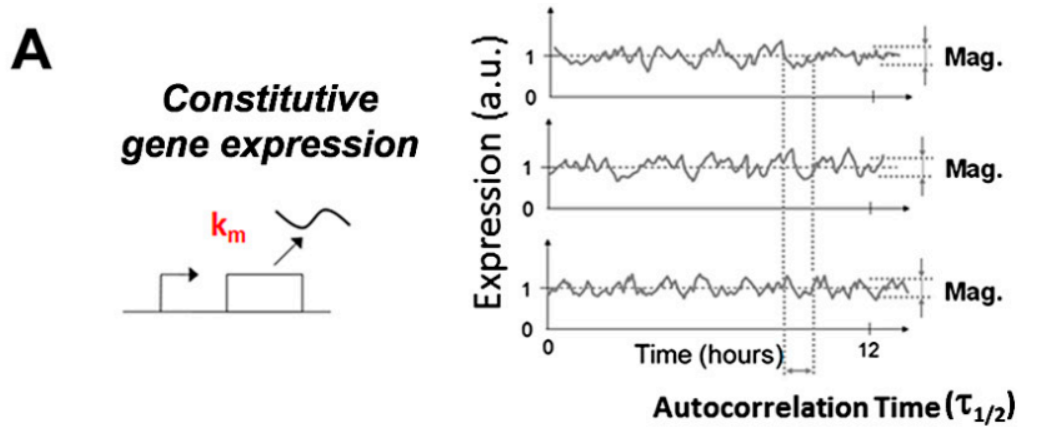
\includegraphics[width=7cm]{burst-1.png}
\end{figure}
\end{textblock*}

\begin{textblock*}{7cm}(8cm,1.5cm)
\begin{figure}
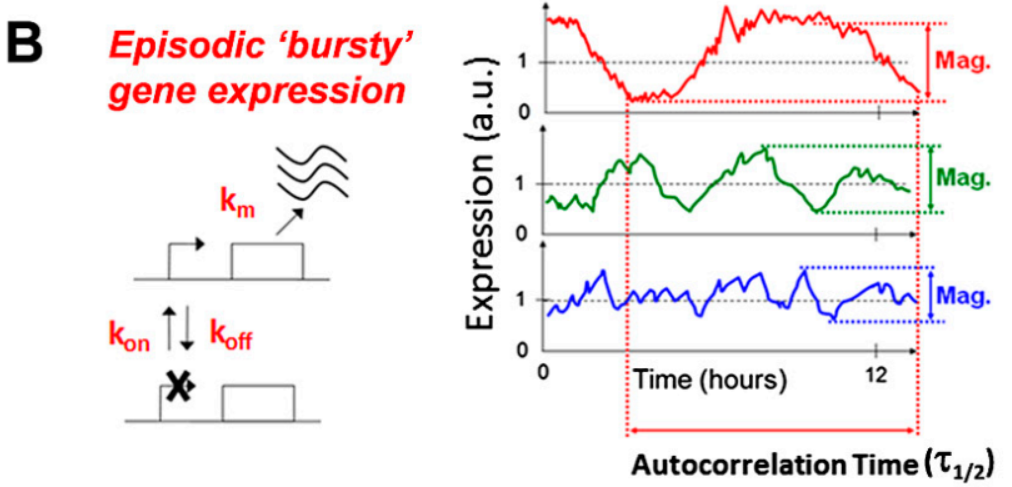
\includegraphics[width=7cm]{burst-2.png}
\end{figure}
\end{textblock*}


\begin{textblock*}{15cm}(0.5cm,6cm)
\begin{itemize}
\item Non-equilibrium expression cannot be measured directly with \emph{ensemble snapshots}
\item Tracking counts in live cells limits the number of species considered simultaneously
\item If the biochemical network is known a-priori, we can build parametric dynamical models
\item Bayesian inference allows us to fit parametric dynamical models without continuous dynamical trajectories
\end{itemize}
\end{textblock*}


\end{frame}

\begin{section}{Modeling stochastic biochemical reaction networks}

\begin{frame}{Stochastic biochemical reaction networks: the repressilator}
\begin{textblock*}{10.5cm}(3cm,1cm)
\begin{figure}
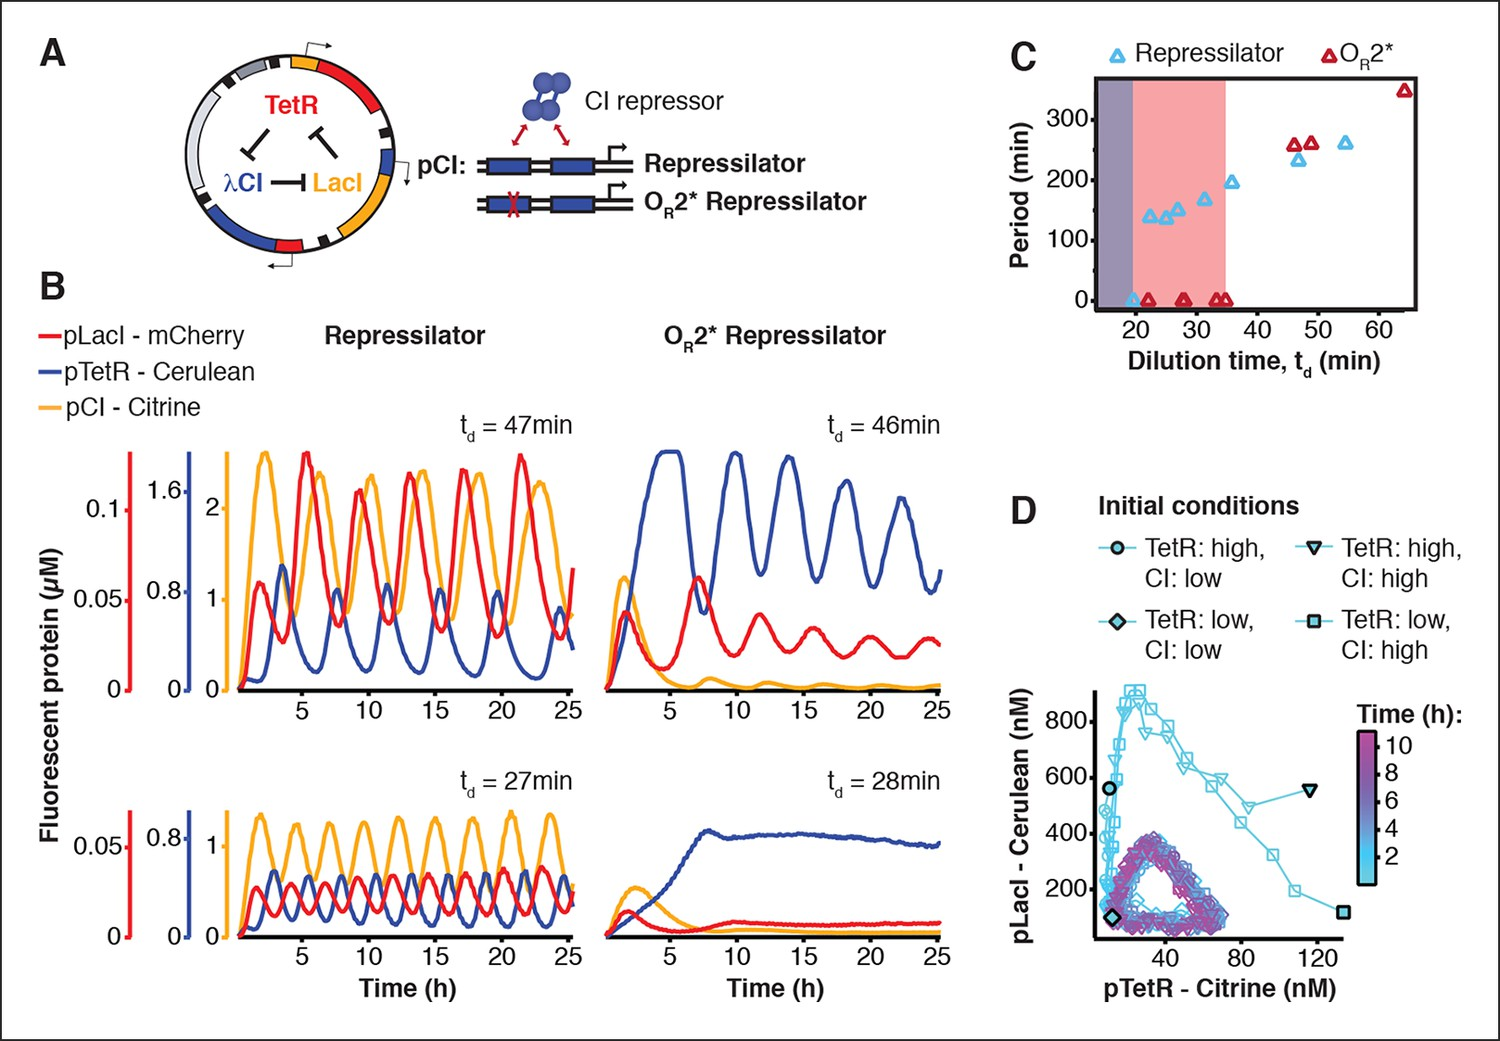
\includegraphics[width=10.5cm]{repressilator.jpg}
\caption{Niederholtmyer et al., eLife 2015}
\end{figure}
\end{textblock*}
\end{frame}



\begin{frame}{Bayesian parameter inference for gene regulation}

Suppose we have a series of ensemble snapshots of an \emph{in-vitro} population:

\begin{align*}
\mathcal{D} = \{\mathcal{D}^{0}, ..., \mathcal{D}^{t}\}
\end{align*}

with $\mathcal{D}^{t} = \{d_{1}, ..., d_{n}\}$. We would like to use $\mathcal{D}$ to fit a dynamical model $\mathcal{M}(\theta)$\\
\vspace{0.2in}
Bayesian inference lets us infer $\theta$ from $\mathcal{D}$ while quantifying the uncertainty in our estimate:

\begin{align*}
P(\theta|\mathcal{D}) \propto P(\mathcal{D}|\theta)P(\theta) = P(\theta)\prod_{n,t} P(\mathcal{D}_{n}^{t}|\theta)
\end{align*}

The likelihood $P(\mathcal{D}_{n}^{t}|\theta)$ is often difficult to define or intractable to compute due to the curse of dimensionality

\end{frame}

\end{section}

\begin{frame}{Estimating the likelihood}

If all reactions take place in a well-mixed solution (Markov), the chemical master equation (CME) applies\\
\begin{align*}
\frac{dP(\mathbf{x},t)}{dt} = \sum_{j} a_{j}(\mathbf{x}-\nu_{j}|\theta)P(\mathbf{x}-\nu_{j},t) - a_{j}(\mathbf{x}|\theta)P(\mathbf{x},t)
\end{align*}
$P(\mathcal{D}^{t}|\theta)$ is the solution to the master equation $P(\mathbf{x},t)$ under parameterization $\theta$\\
\vspace{0.2in}
ABC methods simulate data $\tilde{\mathcal{D}}$ from $\mathcal{M}(\theta)$ using the Gillespie algorithm and compute a distance metric $d(\mathcal{D},\tilde{\mathcal{D}})$ or $d(\mathcal{S}(\mathcal{D}),\mathcal{S}(\tilde{\mathcal{D}}))$ where $\mathcal{S}$ is a summary statistic to approximate the likelihood\\
\vspace{0.2in}
\textcolor{red}{Both suffer from the curse of dimensionality}\\
\vspace{0.2in}

\end{frame}

\begin{frame}{Beating the curse of dimensionality to compute the likelihood}
Deep networks are known to be capable of circumventing the curse. They can model very high-dimensional joint distributions e.g., distributions over images\\
\vspace{0.2in}
Can we use a deep network to perform the map $\Theta\in \mathbb{R}^{n} \rightarrow f(\Theta) = P(\mathcal{D}|\Theta) \in \mathbb{R}^{n+1}$ i.e., compute the likelihood?
\end{frame}

\begin{section}{Application to chemotherapy resistance in melanoma}
\begin{frame}{Drug-induced
reprogramming as a mode of cancer drug resistance}

\begin{textblock*}{12cm}(2cm,1cm)
\begin{figure}
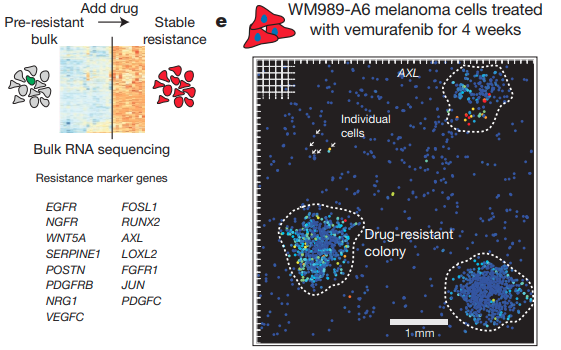
\includegraphics[width=12cm]{resistance.png}
\caption{Shaffer et al., Nature 2017}
\end{figure}
\end{textblock*}

\end{frame}

\begin{frame}{WM989-A6 RNA-FISH data summary}

\begin{textblock*}{15cm}(0.5cm,1cm)
\begin{figure}
\includegraphics[width=15cm]{data-summary.png}
\end{figure}
\end{textblock*}

\end{frame}

\begin{frame}{Graphical abstract}

\begin{textblock*}{14cm}(1.15cm,1.5cm)
\begin{figure}
\captionsetup{font={footnotesize,it}}
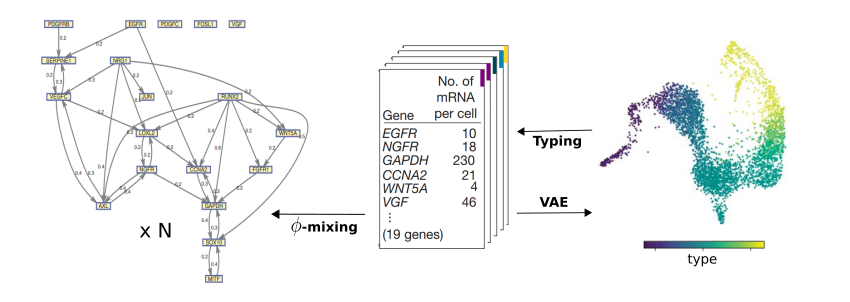
\includegraphics[width=14cm]{sketch.png}
\caption{Gene expression matrices used as training data to learn a latent-space representation of gene expression, uncovering latent structure of the joint distribution and permitting cell typing, account for batch variability. Type information is then used for inference of the underlying regulatory network using the phi-mixing coefficient, which may differ across types}
\end{figure}
\end{textblock*}

\end{frame}
\end{section}

\begin{frame}{Training on BBBC039 U2OS Cells}
\vspace{0.1in}
BBBC039: 200 images, 160 train + 40 validation, 256\;x\;256 random crop

\begin{center}
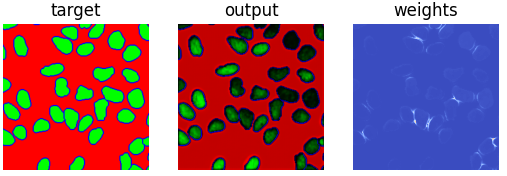
\includegraphics[width=0.8\textwidth]{weights.png}
\end{center}

We train a 3-channel semantic segmentation model with \textbf{weighted} cross-entropy loss:

\begin{equation*}
\mathcal{L} = \sum_{i,j} w_{ij}\log p_{ij}(\tilde{x}) = \sum_{i,j} w_{ij}\log \frac{\exp(-s_{ij}(\tilde{x}))}{\sum_{x\in\chi} \exp(-s_{ij}(\tilde{x}))}
\end{equation*}

$p_{ij}$ is the probability the model assigns a pixel to the true class $\tilde{x} \in \{\textrm{a}, \textrm{b}, \textrm{c}\}$

\end{frame}

\begin{frame}{Training on BBBC039 U2OS Cells}

\begin{center}
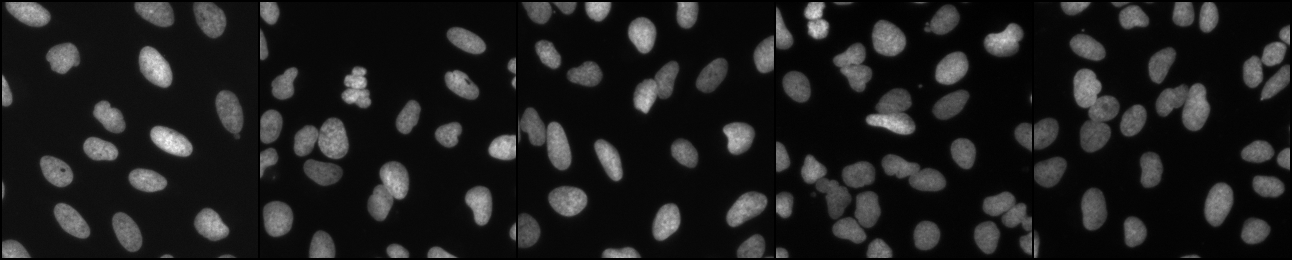
\includegraphics[width=0.85\textwidth]{input-train.png}
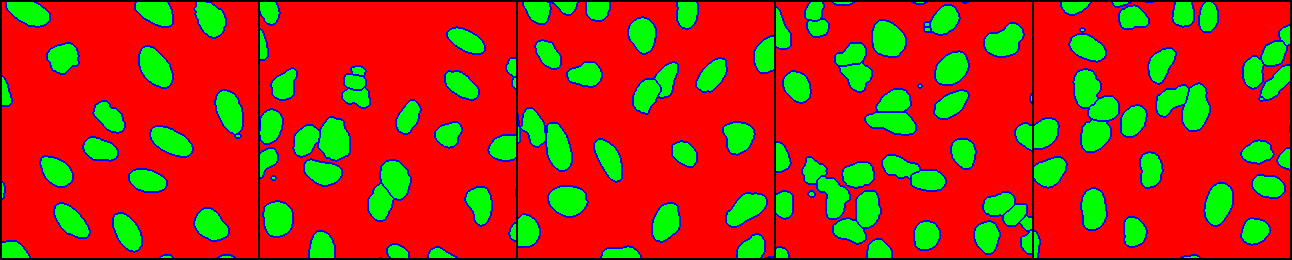
\includegraphics[width=0.85\textwidth]{target-train.png}
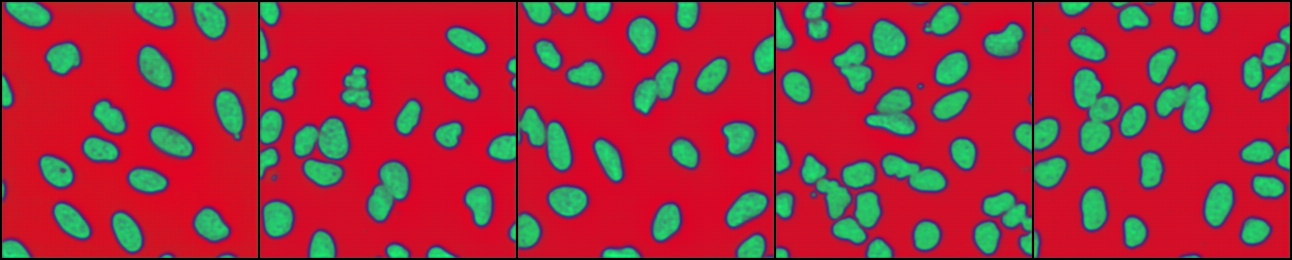
\includegraphics[width=0.85\textwidth]{output-train.png}
\end{center}

\end{frame}

\begin{frame}{Training on BBBC039 U2OS Cells}
Learning rate $\eta=0.01$, Batch-size $B=5$ (32 train iterations, 8 validation)
\begin{center}
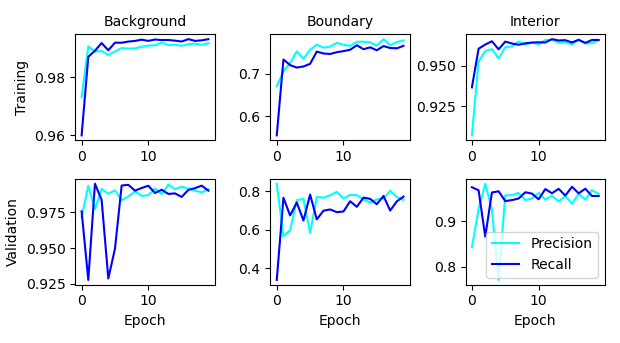
\includegraphics[width=0.85\textwidth]{metrics.png}
\end{center}

\end{frame}



% Adding the option 'allowframebreaks' allows the contents of the slide to be expanded in more than one slide.
\begin{frame}[allowframebreaks]{References}
	\tiny\bibliography{references}
	\bibliographystyle{apalike}
\end{frame}

\end{document}
